\documentclass[conference]{IEEEtran}
\IEEEoverridecommandlockouts

\usepackage{amsmath}
\usepackage{graphicx}
\usepackage{booktabs}
\usepackage{array}
\usepackage{hyperref}
\usepackage{tikz}
\usetikzlibrary{arrows.meta,positioning,shapes.geometric}
\emergencystretch=2em

% Auto-extracted numbers/figures from repo artifacts (do not hand-edit).
% AUTO-GENERATED by scripts/build_paper_artifacts.py. DO NOT EDIT BY HAND.
\newcommand{\RepoCommitSha}{12af321b636fcb6474d09f214d6c1b4afc01adcc}
\newcommand{\NumSubjects}{2}
\newcommand{\ActionAccMean}{83.49}
\newcommand{\ActionAccSD}{0.50}
\newcommand{\ActionAccMin}{82.95}
\newcommand{\ActionAccMax}{83.94}
\newcommand{\FingerAccMean}{82.37}
\newcommand{\FingerAccSD}{4.40}
\newcommand{\FingerAccMin}{79.12}
\newcommand{\FingerAccMax}{87.37}
\newcommand{\ActionECEMean}{0.0341}
\newcommand{\ActionECESD}{0.0378}
\newcommand{\FingerECEMean}{0.0528}
\newcommand{\FingerECESD}{0.0042}
\newcommand{\AgeMean}{16.0}
\newcommand{\AgeSD}{0.0}
\newcommand{\AgeMin}{16}
\newcommand{\AgeMax}{16}
\newcommand{\WindowSec}{0.250}
\newcommand{\HopSec}{0.050}
\newcommand{\TargetFsHz}{256.0}
\newcommand{\ModelParamCount}{27673}
\newcommand{\TrialIdUniqueMin}{1}
\newcommand{\TrialIdUniqueMax}{1}
\newcommand{\BlockIdUniqueMin}{1}
\newcommand{\BlockIdUniqueMax}{1}


\newcommand{\NotAvailable}{\textit{not available}}

\title{
Beyond the Grip:
AlphaHand for Individual Finger Movement Identification from Consumer EEG
}

\author{
\IEEEauthorblockN{\textbf{Jonathan Davanzo}}
\IEEEauthorblockA{
\normalfont\footnotesize First author and lead researcher\\
Summit High School\\
jonathandavanzo@alphahand.org}
\and
\IEEEauthorblockN{\textbf{Liam Bales}}
\IEEEauthorblockA{
\normalfont\footnotesize Summit High School\\
liam.c.bales@gmail.com}
\and
\IEEEauthorblockN{\textbf{Oliver Buchanan}}
\IEEEauthorblockA{
\normalfont\footnotesize Summit High School\\
oliverpbuchanan@icloud.com}
}

\begin{document}
\maketitle

\begin{abstract}
Finger-level assistive control from consumer EEG is difficult because the signal is noisy, low-density, and only indirectly related to hand kinematics. We present AlphaHand, a provenance-preserving Muse 2 pipeline that records timestamp-aligned EEG and event markers, extracts \WindowSec~s windows, trains a calibrated multi-head CNN+LSTM, and evaluates predictions through the same conservative command gates used for robotic-hand actuation. The featured subject-specific 2-M16 deployment checkpoint, trained from two movement sessions and one auxiliary REST session, reached \FeaturedActionAcc\% held-out action accuracy, \FeaturedFingerAcc\% deployment-consistent finger accuracy on true non-REST windows, and \FeaturedJointAcc\% joint action--finger accuracy under deterministic evaluation. In pseudo-live replay, the command path achieved \FeaturedReplayPrecision\% non-REST precision across \FeaturedReplayPositiveSendWindows{} emitted positive windows and hit \FeaturedReplayEventHitRate\% of \FeaturedReplayEventCount{} movement events at \FeaturedReplayLatencyMedianMs{} ms median first-command latency; window-level send recall was \FeaturedReplayRecall\%, reflecting conservative stability gates rather than classifier error alone. False actuation on REST was rare, with \FeaturedReplayFalseActuationCount{} of \FeaturedReplayRestWindows{} true REST windows actuated, supporting an auditable subject-specific demonstration while leaving prospective multi-subject and live-loop validation as future work.
\end{abstract}

\section{Introduction}

Limb loss affects a large population in the United States and is accompanied by substantial functional and psychological burden \cite{ZieglerGraham2008,Singh2024Depression}. Restoring useful hand function therefore requires more than binary grasp detection. Many daily tasks depend on which finger moves and when it moves, making finger-level intent decoding a demanding and clinically meaningful target.

EMG is a standard control modality for practical upper-limb prostheses \cite{Scheme2011EMG}. It is effective when informative residual musculature is available, but it does not directly address users with limited peripheral control signals. For users with limited or absent residual musculature, consumer EEG offers a fundamentally different access path, one that does not depend on peripheral motor signals at all, rather than simply a lower-cost alternative to clinical hardware. Its limitations are severe: the signal is spatially blurred, sensitive to motion and impedance variation, and especially constrained on consumer headsets with only a few dry electrodes. The value of this setting is not that consumer EEG is an ideal sensing modality, but that it tests whether a low-cost, low-channel system can preserve enough usable intent structure to support conservative assistive control. Finger-level decoding from such hardware is therefore a stringent test of whether low-cost brain-computer interfaces can move beyond coarse command vocabularies.

Prior EEG work has shown that deep networks can improve within-subject decoding performance, including the Deep ConvNet family and the compact EEGNet architecture \cite{Schirrmeister2017Deep,Lawhern2018EEGNet}. Consumer devices in the Muse family have also been validated for selected research use cases, including ERP studies and spectral analysis \cite{Krigolson2017Muse,Cannard2021Muse}. At the task level, noninvasive studies have demonstrated that individual finger movements or wrist-vs.-finger movements can be discriminated from EEG under controlled conditions \cite{Liao2014FingerEEG,Mohamed2011WristFinger}. Xiao and Ding further showed that spectral-structure features from high-density EEG improve finger-movement detection and carry discriminative information for individual fingers beyond classic mu/beta features \cite{XiaoDing2015FingerSpectral}. These results establish that EEG contains task-relevant finger information. AlphaHand studies a more constrained deployment setting: high-density sensing is replaced by a four-channel consumer headset, and offline predictions must survive calibration, safety gates, and replay through the command path. Because transfer across users remains a persistent challenge in EEG-BCI, the present manuscript evaluates a subject-specific deployment chain rather than claiming subject-independent generalization \cite{Wu2022Transfer}. We did not attempt subject-independent transfer here because the present manuscript reports one complete deployment evidence chain; the archive does not yet contain matched, prospectively constructed datasets across subjects. Once a classifier is connected to hardware, calibration and uncertainty are operational concerns, not post-hoc cosmetics \cite{Gal2016Dropout,Guo2017Calibration}.

\begin{table*}[t]
\centering
\scriptsize
\setlength{\tabcolsep}{3pt}
\caption{Context against prior noninvasive EEG finger-movement studies. Metrics are not direct benchmarks because task definitions, sensors, and validation protocols differ.}
\label{tab:related-work}
\resizebox{\textwidth}{!}{%
\begin{tabular}{>{\raggedright\arraybackslash}p{0.15\textwidth}>{\raggedright\arraybackslash}p{0.28\textwidth}>{\raggedright\arraybackslash}p{0.25\textwidth}>{\raggedright\arraybackslash}p{0.24\textwidth}}
\toprule
Study & Setup & Reported result & Relevance to AlphaHand \\
\midrule
Mohamed et al. \cite{Mohamed2011WristFinger} & EEG wrist/finger movement imagery and execution; ICA, ERD/ERS features, MD/ANN classifiers. & 65\% MD and 71\% ANN average accuracy. & Coarse wrist-vs.-finger context, not individual-finger decoding. \\
Liao et al. \cite{Liao2014FingerEEG} & 128-channel EEG, 50-channel decoding set, ten usable subjects, pairwise one-hand finger decoding. & 77.11\% average pairwise EEG accuracy; resting-control data near guessing. & High-density offline finger-pair benchmark. \\
Xiao and Ding \cite{XiaoDing2015FingerSpectral} & 128-channel EEG; spectral PCA compared with classic mu/beta PSD features. & 90--91\% movement-vs.-rest detection; 39.7\% five-finger PC accuracy versus 23.3\% mu/beta PSD. & Shows spectral structures carry finger-specific information with far richer sensing than Muse 2. \\
AlphaHand (this work) & Four-channel Muse 2, subject-specific CNN+LSTM, action-conditioned finger decoding, gated replay. & \FeaturedActionAcc\% action accuracy, \FeaturedFingerAcc\% non-REST finger accuracy, \FeaturedReplayPrecision\% pseudo-live non-REST precision. & Low-density, subject-specific, deployment-gated command-path demonstration. \\
\bottomrule
\end{tabular}%
}
\end{table*}

This study does not test whether a four-channel consumer headset can outperform high-density EEG, nor whether the result transfers across users. Instead, it tests whether enough subject-specific structure remains in a sparse consumer montage to survive calibration, safety gating, and replay through an auditable command path. For assistive control, the relevant deployment question is not only whether each window is classified correctly, but whether the system emits correct commands at the right moments while suppressing unsafe movement during REST.

This paper asks a concrete deployment question: can a four-channel consumer EEG headset support an auditable, subject-specific path from EEG window to conservative robotic-hand command? We make three contributions:
\begin{itemize}
\item An end-to-end consumer EEG pipeline for finger-level control, spanning Muse 2 acquisition, timestamp-aligned labeling, fixed-window extraction, subject-specific CNN+LSTM training, calibration, deterministic evaluation, and optional robotic-hand actuation.
\item A deployment-consistent evaluation protocol that reports not only held-out accuracy, but also command-path precision, event hit rate, latency, and false REST actuation under pseudo-live replay.
\item A provenance account for the featured 2-M16 result, including session merging, REST pruning, window counts, saved run outputs, and explicit evidence limits.
\end{itemize}
The manuscript reports the March 19, 2026 2-M16 bundle as the featured result throughout. The scope is deliberately subject-specific: the paper evaluates whether consumer EEG can sustain conservative finger-level control when the full evidence chain, calibration path, and deployment gates are preserved.

\section{Methods}
\subsection{Pipeline Overview}

The pipeline has seven saved stages. Acquisition records raw Muse samples with event markers; window extraction converts recordings into labeled fixed-length examples; training saves model checkpoints and calibrated test predictions; deterministic evaluation computes metrics and command-path summaries; calibration review generates reliability and uncertainty outputs; live inference optionally sends gated commands to the robotic hand; and post-live review converts prediction logs into auditable segments. Figure~\ref{fig:pipeline} summarizes the offline and online paths used in this paper. All manuscript tables are generated from the saved outputs associated with these stages.

\begin{figure}[t]
\centering
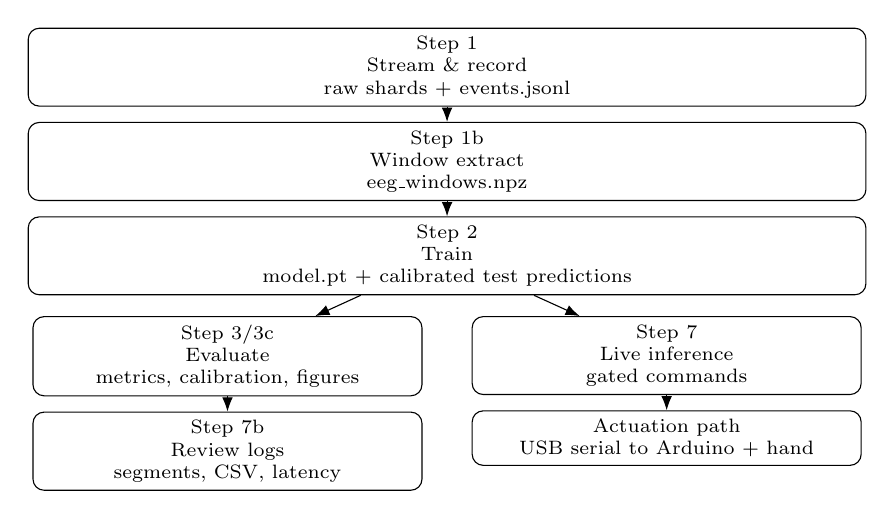
\begin{tikzpicture}[
  node distance=0.55em,
  box/.style={draw, rounded corners, align=center, inner sep=3pt, font=\scriptsize, text width=0.86\columnwidth},
  branch/.style={box, text width=0.39\columnwidth},
  arr/.style={-{Latex[length=1.8mm]}, line width=0.4pt}
]
\node[box] (s1) {Step 1\\Stream \& record\\raw shards + events.jsonl};
\node[box, below=of s1] (s1b) {Step 1b\\Window extract\\eeg\_windows.npz};
\node[box, below=of s1b] (s2) {Step 2\\Train\\model.pt + calibrated test predictions};
\node[branch, below=0.75em of s2, xshift=-0.23\columnwidth] (s3) {Step 3/3c\\Evaluate\\metrics, calibration, figures};
\node[branch, below=0.75em of s2, xshift=0.23\columnwidth] (s7) {Step 7\\Live inference\\gated commands};
\node[branch, below=of s3] (s7b) {Step 7b\\Review logs\\segments, CSV, latency};
\node[branch, below=of s7] (act) {Actuation path\\USB serial to Arduino + hand};
\draw[arr] (s1) -- (s1b);
\draw[arr] (s1b) -- (s2);
\draw[arr] (s2) -- (s3);
\draw[arr] (s2) -- (s7);
\draw[arr] (s3) -- (s7b);
\draw[arr] (s7) -- (act);
\end{tikzpicture}
\caption{End-to-end system flow and saved outputs. The online branch can transmit gated commands over USB serial to an Arduino-linked five-finger robotic hand. Quantitative results reported in this paper are extracted from archived stage outputs rather than manual transcription.}
\label{fig:pipeline}
\end{figure}

\subsection{Data Acquisition and Persistence}

\subsubsection{Human Subjects and Ethics}

Recordings were collected under IRB approval permitting enrollment of participants ages 16 and older. All participants provided written consent or assent; written parent or guardian consent was obtained for minors. The featured 2-M16 participant was a study-team self-subject; protocol familiarity may therefore improve compliance, reduce motion, and inflate performance relative to users unfamiliar with the protocol. The broader project archive contains recordings from approximately 20 consented participants, ages 16--60, male and female, including students, teachers, and parents. Most archived recordings are smaller, lack trained checkpoints, are quality-flagged, or are missing the full REST and deployment evidence chain required for the present analysis. Quantitative claims in this manuscript are therefore limited to the featured 2-M16 deployment bundle.

\subsubsection{Hardware}

The data analyzed here were acquired with a Muse 2 headset (Muse/InteraXon Inc., Toronto, ON, Canada), configured as a four-channel wearable EEG system (TP9, AF7, AF8, TP10) at \TargetFsHz~Hz \cite{Muse2Official}. This hardware defines the central constraint of the study: finger-level decoding from a consumer headset rather than from a research-grade cap \cite{Krigolson2017Muse,Cannard2021Muse}.

\subsubsection{EEG Artifact-Minimizing Recording Protocol}

During recording, subjects were seated, relaxed, and instructed to keep gaze fixed on the task point while avoiding non-task movements. The operator monitored stream health, electrode connectivity, and general system status live, with breaks used when needed. These controls were intended to reduce motion, gaze, and connectivity-related artifacts at recording time. They should not be interpreted as equivalent to dedicated EMG/EOG monitoring or post-hoc ICA-based artifact rejection; this limitation is revisited in Section~\ref{sec:limitations}.

\subsubsection{Streaming Model}

All EEG samples are timestamped in the LSL clock domain, and event timestamps are converted into the same timebase before labeling. Absolute session time is defined as:

\[
t_{\text{session}} = t_{\text{lsl}} - t_{\text{stream\_start}}
\]

\subsubsection{Persistence Architecture}

Raw EEG samples are stored first as NumPy shards to preserve sample fidelity and avoid rounding error from CSV serialization. Event markers are written to both a legacy CSV view and an authoritative \texttt{events.jsonl} file. The analysis in this paper uses the JSONL event log as the canonical label source.

\subsubsection{Cohort Summary}
Demographics, dataset duration, and event label counts are extracted directly from saved metadata. Table~\ref{tab:demo} reports the featured participant metadata, and Table~\ref{tab:sessions} reports dataset provenance. The featured 2-M16 run uses a filtered derived dataset assembled from two movement sessions and one auxiliary REST session; \FeaturedDerivedRemovedN{} of \FeaturedDerivedSourceN{} extracted windows were removed, leaving \FeaturedDerivedKeptN{} windows for the final dataset. Table~\ref{tab:events} reports the raw-session event counts underlying that dataset, and Fig.~\ref{fig:featured-provenance} summarizes the full data path for the featured 2-M16 result.

The 2-M16 REST pruning criterion is recorded in the saved filter manifest: REST event IDs 0, 1, and 2 from session 2-M16\_20260216\_150056\_01 were removed because they were repeatedly inferred as movement or dominated held-out REST failures during dataset-quality review. Because the pruning rule is recorded in the saved filter manifest and the featured training configuration points to the already-filtered derived dataset, the reported model was trained and evaluated only after this dataset-quality decision had been applied.

% AUTO-GENERATED by scripts/build_paper_artifacts.py. DO NOT EDIT BY HAND.
\begin{table}[t]
\centering
\caption{Subject demographics (from \texttt{subject.json}; sex inferred from subject ID when missing).}
\label{tab:demo}
\begin{tabular}{llll}
\toprule
Subject & Age & Sex & Handedness \\
\midrule
1-M16 500 & 16 & Male & Right \\
2-M16 & 16 & Male & Right \\
\bottomrule
\end{tabular}
\end{table}


\begin{table}[t]
\centering
\scriptsize
\setlength{\tabcolsep}{3pt}
\caption{Session durations and write integrity (computed from \texttt{run\_meta.json}).}
\label{tab:sessions}
\resizebox{\columnwidth}{!}{%
\begin{tabular}{p{0.30\linewidth}rrrr}
\toprule
Session & Samples recv. & Samples written & Drop (\%) & Duration (min) \\
\midrule
1-M16 500\_\allowbreak20260216\_\allowbreak123857\_\allowbreak01 & 818208 & 818208 & 0.00 & 53.3 \\
2-M16\_\allowbreak20260216\_\allowbreak150056\_\allowbreak01 & 799740 & 799740 & 0.00 & 52.1 \\
\bottomrule
\end{tabular}%
}
\end{table}


\begin{table*}[t]
\centering
\scriptsize
\caption{Raw-session event label counts for the recorded sessions underlying the featured 2-M16 dataset. Role indicates a movement session merged into the derived dataset (Core) or an auxiliary REST-only session added for REST coverage (Aux REST). Column headers abbreviate thumb/index/middle/ring/pinky open and close events.}
\label{tab:events}
\setlength{\tabcolsep}{4pt}
\begin{tabular}{lllrrrrrrrrrrr}
\toprule
Subject & Session & Role & \shortstack{REST} & \shortstack{TH\\OPEN} & \shortstack{TH\\CLOSE} & \shortstack{IN\\OPEN} & \shortstack{IN\\CLOSE} & \shortstack{MID\\OPEN} & \shortstack{MID\\CLOSE} & \shortstack{RING\\OPEN} & \shortstack{RING\\CLOSE} & \shortstack{PINK\\OPEN} & \shortstack{PINK\\CLOSE} \\
\midrule
2-M16 & 2-\allowbreak{}M16\_\allowbreak{}20260216\_\allowbreak{}150056\_\allowbreak{}01 & Core & 5 & 58 & 55 & 54 & 57 & 55 & 59 & 57 & 60 & 60 & 59 \\
2-M16 & 2-\allowbreak{}M16\_\allowbreak{}20260317\_\allowbreak{}190134 & Core & 10 & 1 & 2 & 2 & 3 & 3 & 2 & 1 & 3 & 2 & 3 \\
2-M16 & 2-\allowbreak{}M16\_\allowbreak{}20260315\_\allowbreak{}145838\_\allowbreak{}01 & Aux REST & 8 & 0 & 0 & 0 & 0 & 0 & 0 & 0 & 0 & 0 & 0 \\
\bottomrule
\end{tabular}
\end{table*}



\begin{figure*}[t]
\centering
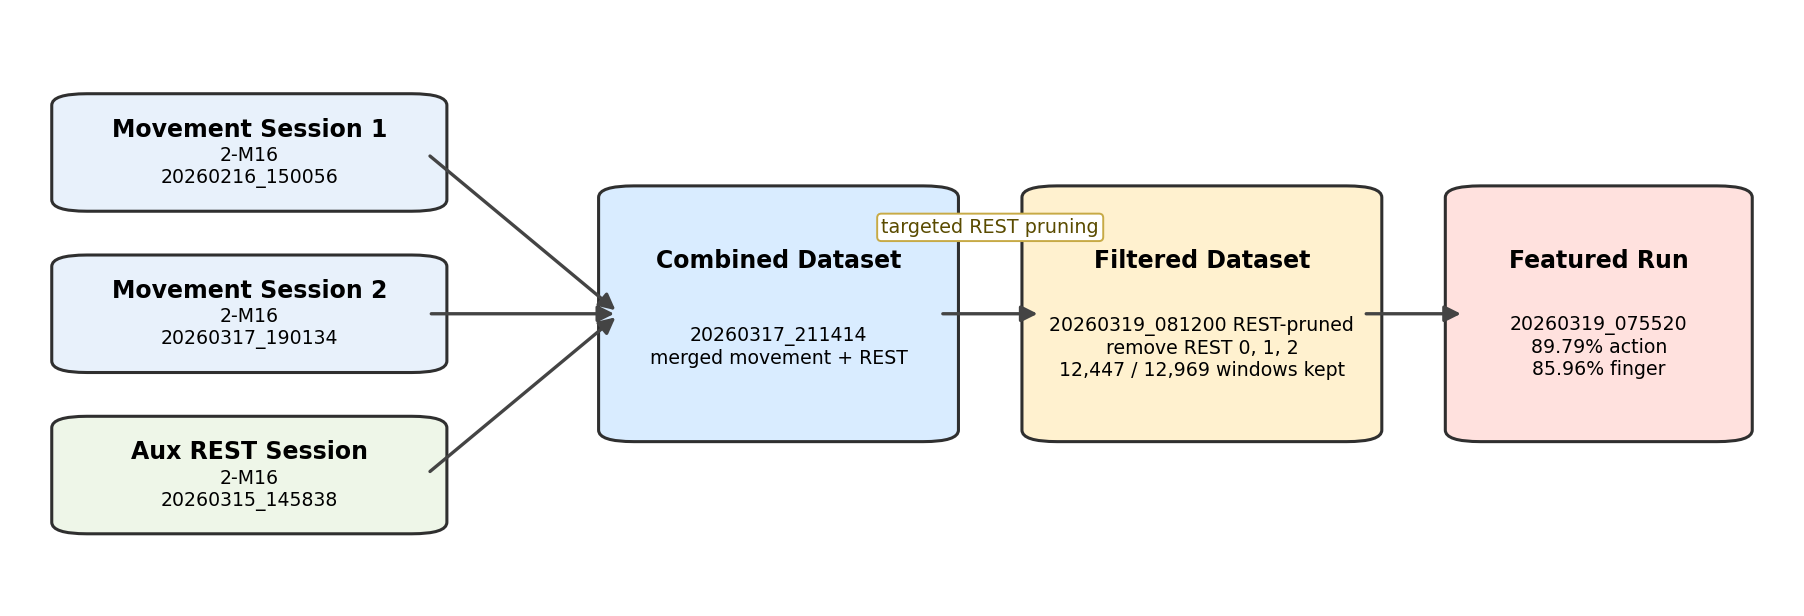
\includegraphics[width=\textwidth]{../paper_figures/featured_dataset_provenance.png}
\caption{Provenance of the featured 2-M16 result. Two movement sessions and one auxiliary REST session are merged into a combined dataset, targeted REST windows are removed according to the saved filter manifest, and the resulting filtered dataset produces the featured run used throughout the manuscript. The pruning step occurred before model training and evaluation.}
\label{fig:featured-provenance}
\end{figure*}

\subsection{Window Extraction and Leakage Controls}

Sliding windows are extracted with fixed duration \WindowSec~s and hop \HopSec~s, then resampled to a fixed \TargetFsHz~Hz grid. Each window receives one action label and, when appropriate, one finger label. The deployable label space separates action from finger identity: a 5-way active-finger head is trained on non-REST windows, while a binary applicability head predicts whether a finger label is meaningful for the current window. Windows carrying the ambiguous combination OPEN/CLOSE with finger NONE are rejected during extraction rather than passed downstream. Figure~\ref{fig:raw-windowing} grounds the procedure with an event-centered recorded segment and the corresponding overlapping extraction windows.

\begin{figure}[t]
\centering
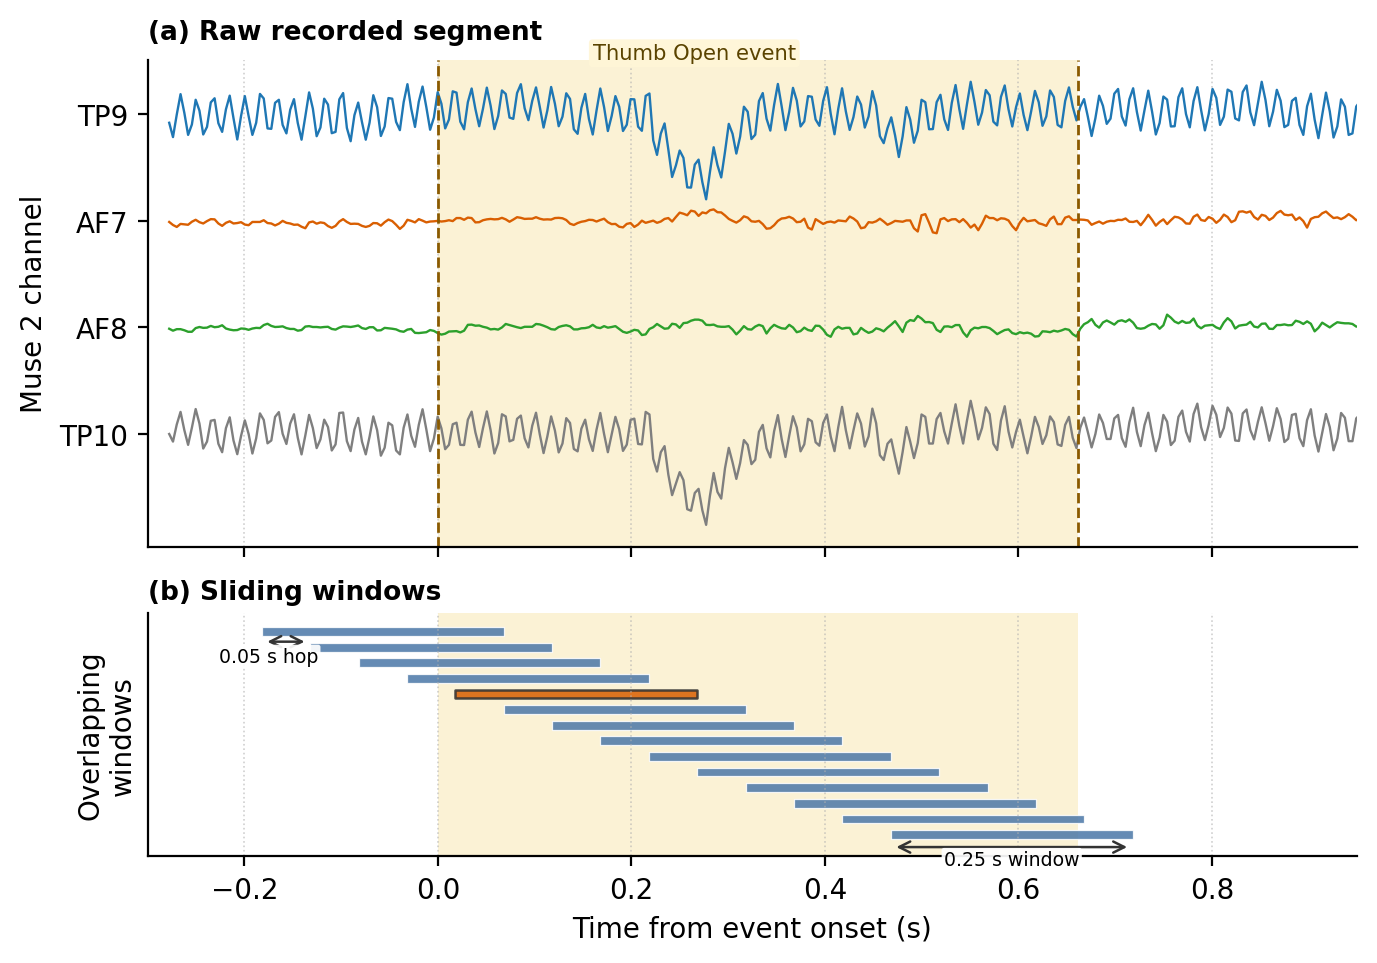
\includegraphics[width=\columnwidth]{../paper_figures/raw_eeg_windowing_example.png}
\caption{Representative event-centered recorded segment from a source session underlying the featured 2-M16 dataset. (a) Raw Muse 2 traces around the labeled event. (b) Overlapping \WindowSec~s extraction windows with \HopSec~s hop over the same interval. The overlap increases the number of labeled training examples, but it also induces temporal dependence between neighboring windows.}
\label{fig:raw-windowing}
\end{figure}

\begin{figure}[t]
\centering
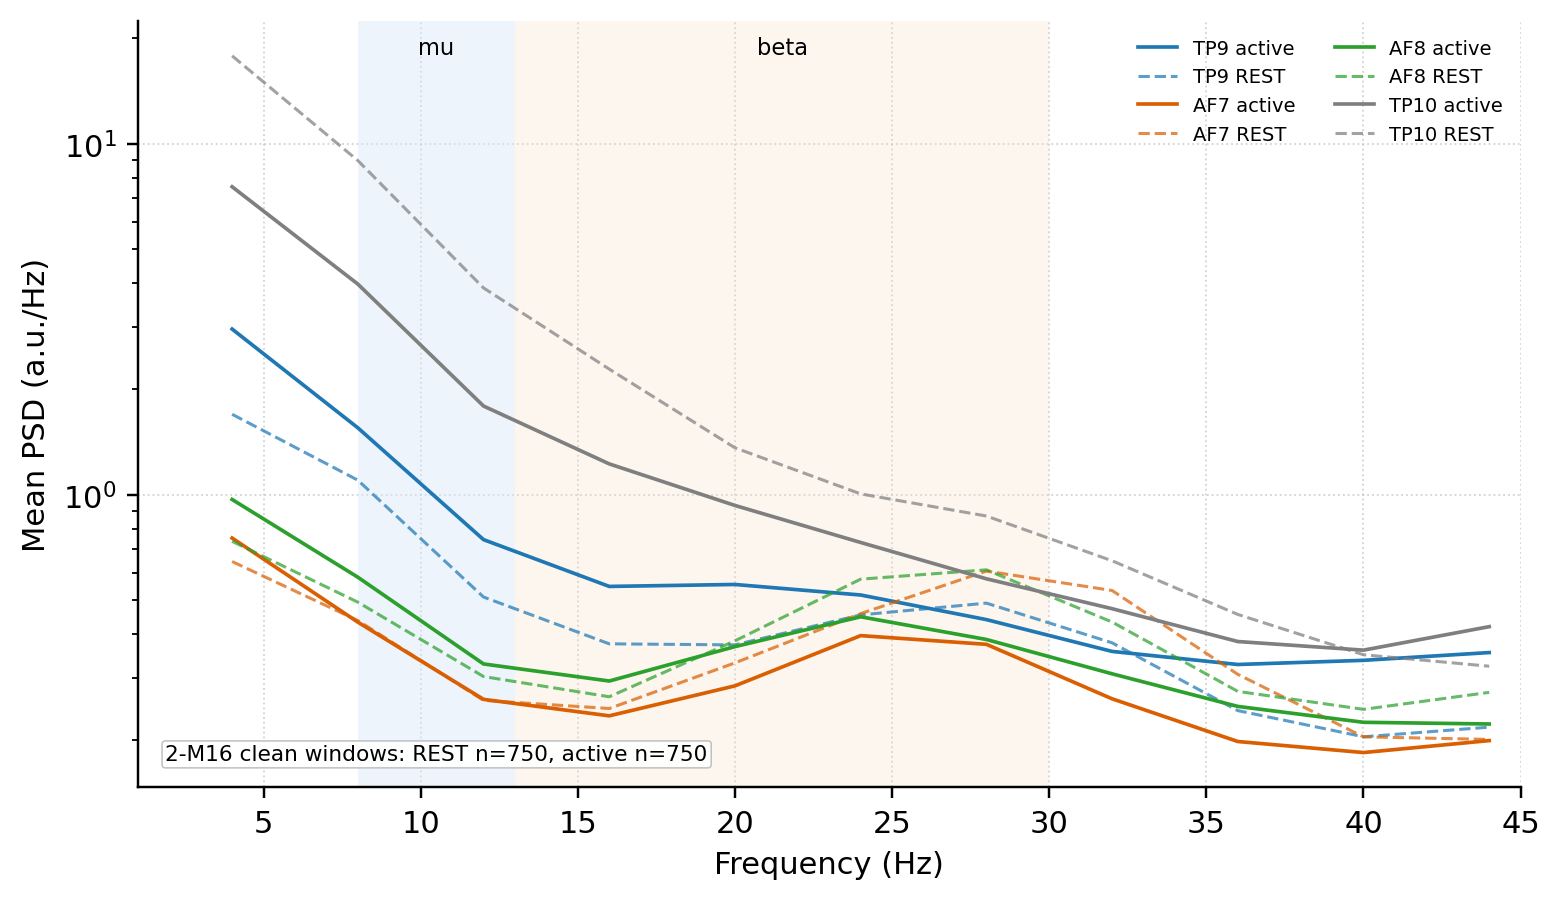
\includegraphics[width=\columnwidth]{../paper_figures/featured_psd_rest_active.png}
\caption{Representative power spectral density from clean windows in the featured 2-M16 dataset. Solid traces average active-movement windows and dashed traces average REST windows for each Muse 2 channel. The panel is descriptive and is intended to ground the low-channel signal regime, not to test a preregistered spectral hypothesis.}
\label{fig:psd}
\end{figure}

The nominal sample count per window is:

\[
N = f_s \times T_{\text{window}} = \TargetFsHz \times \WindowSec = 64~\text{samples}
\]

Windows containing non-finite values are excluded during training. The extracted bundles also store extraction artifact flags and gap flags; the corresponding counts are summarized in Table~\ref{tab:dataset}. No additional EEG artifact-rejection stage beyond the saved extraction checks is documented in the archived outputs analyzed here.

\begin{table*}[t]
\centering
\caption{Dataset and window extraction summary (from \texttt{eeg\_windows.npz} and \texttt{run\_meta.json}).}
\label{tab:dataset}
\begin{tabular}{llrrrrrr}
\toprule
Subject & Session & $N$ windows & Window (s) & Hop (s) & Mean overlap (\%) & Artifacts (count) & Gaps (count) \\
\midrule
1-M16 500 & 1-M16 500\_20260216\_123857\_01 & 13188 & 0.250 & 0.050 & 85.5 & 0 & 0 \\
1-M16 500 & 1-M16 500\_20260216\_123857\_01 & 13188 & 0.250 & 0.050 & 85.5 & 0 & 0 \\
2-M16 & combined\_20260302\_120000 & 10610 & 0.250 & 0.050 & 82.8 & 0 & 0 \\
\bottomrule
\end{tabular}
\end{table*}



\subsubsection{Split Strategy and Leakage Controls}
Training uses a group-aware 80/20 holdout split as recorded in each run configuration. The pipeline asserts no group overlap between train and test windows, supports optional temporal purging, and runs a window-index diagnostic to detect suspicious ordering leakage. In the representative saved outputs, no extra temporal exclusion band is applied around the test windows beyond the group-aware split.

The saved window bundles include trial and block identifier fields, but in the current outputs both are constant across each bundle. Strict trial-level evaluation is therefore not available for the runs reported here. The split logic instead relies primarily on event identifiers and secondary time-based grouping for windows with no event ID. Windows without event IDs arise primarily from REST/background intervals or boundary regions not assigned to a discrete movement event. These windows are grouped by secondary time-based identifiers so that temporally adjacent unlabeled-background windows are not split arbitrarily across train and test sets. REST window counts in the evaluation tables should be interpreted with this windowing scheme in mind: a small number of REST events can still generate many overlapping REST windows.

A post-hoc audit of the cached test indices found no shared \((\mathrm{session\_id}, \mathrm{event\_id})\) groups between test windows and the complementary training/calibration pool for either reported run, and found zero exact duplicate raw windows crossing the train/test boundary. This reduces the risk of direct split leakage, while leaving the temporal dependence created by overlapping windows and adjacent event segments as a statistical limitation.

\subsubsection{Diagnostics and Quality Controls}
The pipeline includes explicit hardening against common streaming-EEG failure modes: non-finite windows are removed before training, group-aware splitting prevents direct group overlap, optional purging can remove windows adjacent in time to test data, and a separate validation stage produces a dataset-quality report for each run.

\subsection{Model and Training}

AlphaHand uses a multi-head CNN+LSTM network with shared temporal features and three prediction heads: a 5-way active-finger head, a 3-way action head, and a binary finger-applicability head. The deployable configuration used in the representative runs includes two temporal 1D convolution blocks (16 and 32 channels; kernel sizes 5 and 3), group normalization, dropout, a single-layer LSTM with hidden size 64, and three linear heads. Each convolution block uses \texttt{GroupNorm(num\_groups=min(4, C\_out))}; because the two blocks have 16 and 32 output channels, both use four groups. The model has \ModelParamCount{} trainable parameters. Before recurrent integration, the convolutional front end spans a 7-sample local temporal receptive field, approximately 27~ms at \TargetFsHz~Hz; the LSTM then integrates information across the full \WindowSec~s window.

\begin{table}[t]
\centering
\caption{CNN+LSTM model configuration for the current deployable active-finger setup.}
\begin{tabular}{lp{0.63\columnwidth}}
\toprule
Component & Setting \\
\midrule
Input & $[T{=}64, C{=}4]$ EEG window \\
Conv1 & 16 channels, kernel 5, dropout 0.3 \\
Conv2 & 32 channels, kernel 3, dropout 0.3 \\
Norm & GroupNorm with $\min(4, C_{\mathrm{out}})$ groups per convolution block \\
LSTM & 1 layer, hidden size 64 \\
Heads & Linear(64$\rightarrow$5) active finger, Linear(64$\rightarrow$3) action, Linear(64$\rightarrow$1) applicability \\
Parameters & \ModelParamCount \\
\bottomrule
\end{tabular}
\end{table}

The loss function is

\[
\mathcal{L} = \mathrm{CE}_{\mathrm{action}} + \lambda_f \, \mathrm{CE}_{\mathrm{finger}}(\mathrm{non\text{-}REST}) + \lambda_a \, \mathrm{BCE}_{\mathrm{applicability}}
\]

where the finger loss is computed only on non-REST windows and the applicability loss is computed on all windows with target \(1[\mathrm{action}\neq \mathrm{REST}]\). The action head additionally supports class weighting, including a configurable REST weight recorded in each run configuration.
For the featured run, \(\lambda_f=1.0\) and \(\lambda_a=0.5\), as recorded in \texttt{train\_config.json}; the action loss weight and REST action weight were both 1.0.

\subsubsection{Training Procedure}
Training hyperparameters are saved in \texttt{train\_config.json} and summarized in Table~\ref{tab:perf}. The featured 2-M16 configuration reports 60 epochs, batch size 64, learning rate 0.001 with no learning-rate scheduler recorded, and Adam optimization. It uses REST action weight 1.0 and action weights [1.0, 1.0, 1.0]. The archived configuration file does not expose separate early-stopping or gradient-clipping settings, so those procedures are not reported as components of the present run.

Input normalization is performed with a per-channel normalizer fit on the training split. A held-out calibration subset of the training data is then used to fit separate scalar temperatures for the action, finger, and applicability heads, and those parameters are saved alongside the trained model.

\subsection{Calibration, Evaluation, and Actuation}
\subsubsection{Monte Carlo Dropout for Uncertainty Estimation}

For MC-dropout uncertainty figures (Step~3c), dropout layers remain active at inference time. For \(K\) stochastic forward passes:

\[
\mu = \frac{1}{K}\sum_{k=1}^{K}\hat{y}_k
\]

\[
\sigma^2 = \frac{1}{K}\sum_{k=1}^{K}(\hat{y}_k - \mu)^2
\]

Reliability diagrams evaluate calibration, while confidence--uncertainty scatter plots visualize uncertainty concentration. Deterministic evaluation uses temperature-scaled test predictions saved after training or recomputed from the archived model and scaler in evaluation mode.

Live inference uses deterministic forward passes, applies saved post-hoc temperature scaling before softmax when available, and keeps MC-dropout analysis out of the Step~7 deployment path. We use ``deployment-consistent'' to mean that evaluation applies the same decode invariants used before actuation: REST predictions map to NONE, OPEN/CLOSE predictions require an active finger, and low-confidence finger/applicability outputs suppress commands rather than rewriting labels. The deployed decode path enforces REST $\Rightarrow$ NONE and OPEN/CLOSE $\Rightarrow$ active finger. Low finger confidence and low applicability act as actuation gates rather than label rewrites.

\subsubsection{Deterministic Evaluation and Calibration}
From each run's saved \texttt{test\_predictions.npz}, we compute ECE with the same convention as the evaluation pipeline: 10 equal-width confidence bins over $[0, 0.1], (0.1, 0.2], \ldots, (0.9, 1.0]$. In the archived predictions, softmax confidences are strictly positive, so assigning the exact boundary value 0.0 to the first bin has no practical effect. Table~\ref{tab:perf} reports action ECE over all test windows and finger ECE over true non-REST windows. The evaluation bundle also reports applicability false-positive and false-negative rates, action--applicability disagreement, and command-path invariants used to validate the deployment decoder.

For the featured run, action ECE is \FeaturedActionECE and finger ECE on true non-REST windows is \FeaturedFingerECE. Lower ECE indicates better agreement between predicted confidence and empirical accuracy; these values should still be interpreted in light of overlapping-window correlation and potential distribution shift between event segments.

\subsubsection{Online Inference and Actuation}
The live inference stage implements online windowing and inference capable of sending actuation commands, but the present bundle supports replay-time command-path reporting rather than a dedicated live-loop latency audit. The command path is intentionally precision-biased. It treats uncertain windows as no-send decisions rather than forcing a best-guess actuation. Postprocessing combines exponential smoothing, action/finger/applicability thresholds, a minimum joint-confidence requirement, a consecutive-window stability gate, and per-finger cooldown/hold intervals. For the featured March 19, 2026 bundle, commands require agreement across \FeaturedActuationStabilityWindows{} consecutive windows (approximately \FeaturedActuationStabilityMs{} ms at a \HopSec~s hop) before they are emitted; the same bundle uses action, finger, and applicability thresholds of 0.05, 0.20, and 0.40, respectively. The cooldown is an actuator-protection interval for the commanded finger, not a global lockout of the hand: other fingers may receive commands during that interval if their own gates pass. The host serial ceiling is 20 commands/s, matching the 50 ms inference hop, and the Arduino receiver enforces per-finger hold timers with non-blocking servo updates. The action threshold is intentionally permissive because REST suppression is dominated by the REST/NONE invariant, finger and applicability gates, stability requirement, and cooldown; archived deployment-selection reports prioritize would-send precision and false REST actuation over offline split accuracy. When actuation is enabled, commands are sent over USB serial to an Arduino-linked five-finger robotic hand. Hardware safety gates prevent actuation whenever the predicted action is REST or the predicted finger is NONE, and the runtime enforces the same REST/NONE and OPEN-or-CLOSE/active-finger pairing used during deterministic evaluation.

Latency-aware adaptation was not part of the reported deployment policy; future versions could adjust thresholds, stability requirements, or command timing based on observed runtime latency.

To make post-live validation auditable, Step~7 prediction logs are postprocessed into compact summaries, contiguous predicted-state segments, and reviewer CSVs. These saved outputs support manual alignment against video or safe shadow-mode robot motion.

Dedicated Step~7 live latency logs are \NotAvailable{} for the present bundle. The paper therefore reports replay-time command-path summaries, but not a complete live-loop latency audit.

\subsubsection{Representative Run Selection and Reproducibility}
The project archive contains more recordings and runs than can be presented compactly in an IEEE-style manuscript, but most runs do not have the same complete evidence chain. Quantitative reporting is therefore restricted to the featured run with archived windows, training configuration, deterministic evaluation, calibration review, and pseudo-live replay. The March 19 2-M16 checkpoint is used as the deployment checkpoint because the model-selection audit prioritized command-path safety: pseudo-live would-send precision, event hit rate, and false REST actuation. A later checkpoint scored higher on some offline metrics, but its replay safety metrics were weaker, so it is not used for the deployment claims in this paper.

All quantitative claims in this paper are extracted directly from saved run outputs. The manuscript uses the archived window dataset, training configuration, summary metrics, calibrated predictions, replay output, and report figures for the featured 2-M16 run. Missing expected saved outputs are reported explicitly as \NotAvailable{}. The additional loss-curve validation figure is generated only when real per-epoch training history is present; because the original deployment checkpoint predates that logging, the displayed curve is labeled as a rerun of the featured recipe rather than as a replacement deployment checkpoint.


\section{Results}

We report three levels of evaluation. First, held-out window metrics test whether the model separates action and finger labels under deterministic inference. Second, deployment-consistent decoding tests whether predictions remain valid after enforcing REST/NONE and active-finger invariants. Third, pseudo-live replay tests whether predictions survive the same stability gates, cooldowns, and command-suppression logic used before robotic actuation. These levels should not be collapsed into a single accuracy number.

Table~\ref{tab:perf} reports the featured March 19, 2026 2-M16 deployment checkpoint. This run is the strongest complete evidence chain and anchors the analysis that follows. It reaches \FeaturedActionAcc\% action accuracy and \FeaturedFingerAcc\% deployment-consistent finger accuracy on \FeaturedNTest{} test windows (\FeaturedNNonRest{} true non-REST), well above uniform-prior chance levels of 33.3\% for three-way action classification and 20\% for five-way finger classification, although class imbalance means these values are reference baselines rather than empirical majority-class baselines. The central test is whether this performance survives the command logic required for actuation.

Only the featured 2-M16 bundle currently includes the paired deterministic evaluation and pseudo-live replay outputs needed to inspect the full command path. In that stricter setting, the model reports \FeaturedJointAcc\% joint action--finger accuracy under deployment-style evaluation and \FeaturedReplayPrecision\% non-REST precision over \FeaturedReplayPositiveSendWindows{} emitted positive windows. Window-level send recall was \FeaturedReplayRecall\%, but this is a deployment-throughput metric rather than a classification accuracy figure. It denotes \FeaturedReplayCorrectSendWindows{} correctly emitted non-REST windows out of \FeaturedReplayNonRestWindows{} true non-REST replay windows and reflects overlapping windows, stability gates, command persistence, duplicate suppression, and cooldown rather than classifier error alone. At the event level, replay hit \FeaturedReplayEventHitRate\% of \FeaturedReplayEventCount{} movement events, with \FeaturedReplayEventMissCount{} misses and \FeaturedReplayLatencyMedianMs{} ms median first-command latency. Critically, only \FeaturedReplayFalseActuationCount{} of \FeaturedReplayRestWindows{} true REST replay windows produced an actuation command, a false actuation rate of \FeaturedFalseActuationRateRest\%. The resulting operating point is conservative: few positive commands are committed, but the commands that pass the gate are usually correct.

\begin{table*}[t]
\centering
\scriptsize
\setlength{\tabcolsep}{3pt}
\caption{Per-subject test performance and calibration (from \texttt{metrics.json} and \texttt{test\_predictions.npz}).}
\label{tab:perf}
\resizebox{\textwidth}{!}{%
\begin{tabular}{lp{0.30\textwidth}rrrrrrrr}
\toprule
Subject & Session & $n_{test}$ & $n_{non\text{-}REST}$ & Action Acc (\%) & 95\% CI & Finger Acc$_{non\text{-}REST}$ (\%) & 95\% CI & Action ECE & Finger ECE$_{non\text{-}REST}$ \\
\midrule
1-M16 500 & 1-M16 500\_\allowbreak20260216\_\allowbreak123857\_\allowbreak01 & 2648 & 2534 & 77.38 & [75.75, 78.93] & 86.27 & [84.87, 87.55] & 0.0815 & 0.0123 \\
2-M16 & combined\_\allowbreak20260302\_\allowbreak120000 & 2457 & 1908 & 82.95 & [81.41, 84.38] & 87.37 & [85.80, 88.78] & 0.0777 & 0.0539 \\
\bottomrule
\end{tabular}%
}
\end{table*}



\subsection{Representative Validation Figures}
For the featured 2-M16 run, the archived Step~3c reliability output includes the action and finger confusion matrices together with calibration summaries, while Table~\ref{tab:perf} reports calibration error from the saved predictions. These views separate quantities that are often collapsed into a single headline number: class confusability, uncertainty concentration, and confidence calibration. Most action errors occur between OPEN and CLOSE rather than between movement and REST, while finger errors concentrate among neighboring non-thumb digits rather than THUMB. A supporting MC-dropout confidence--uncertainty panel shows a dense region of high-confidence, low-uncertainty windows with a thinner diffuse tail, consistent with a gate that suppresses ambiguous commands rather than converting them into actuation. Because the deployment checkpoint predates per-epoch history logging, Figure~\ref{fig:featured-loss-curve} is included only as a training-dynamics sanity check for the same featured recipe, not as evidence replacing the archived deployment checkpoint.

% AUTO-GENERATED by scripts/build_paper_artifacts.py. DO NOT EDIT BY HAND.
\begin{figure*}[t]
\centering
\begin{minipage}[b]{0.49\linewidth}\centering
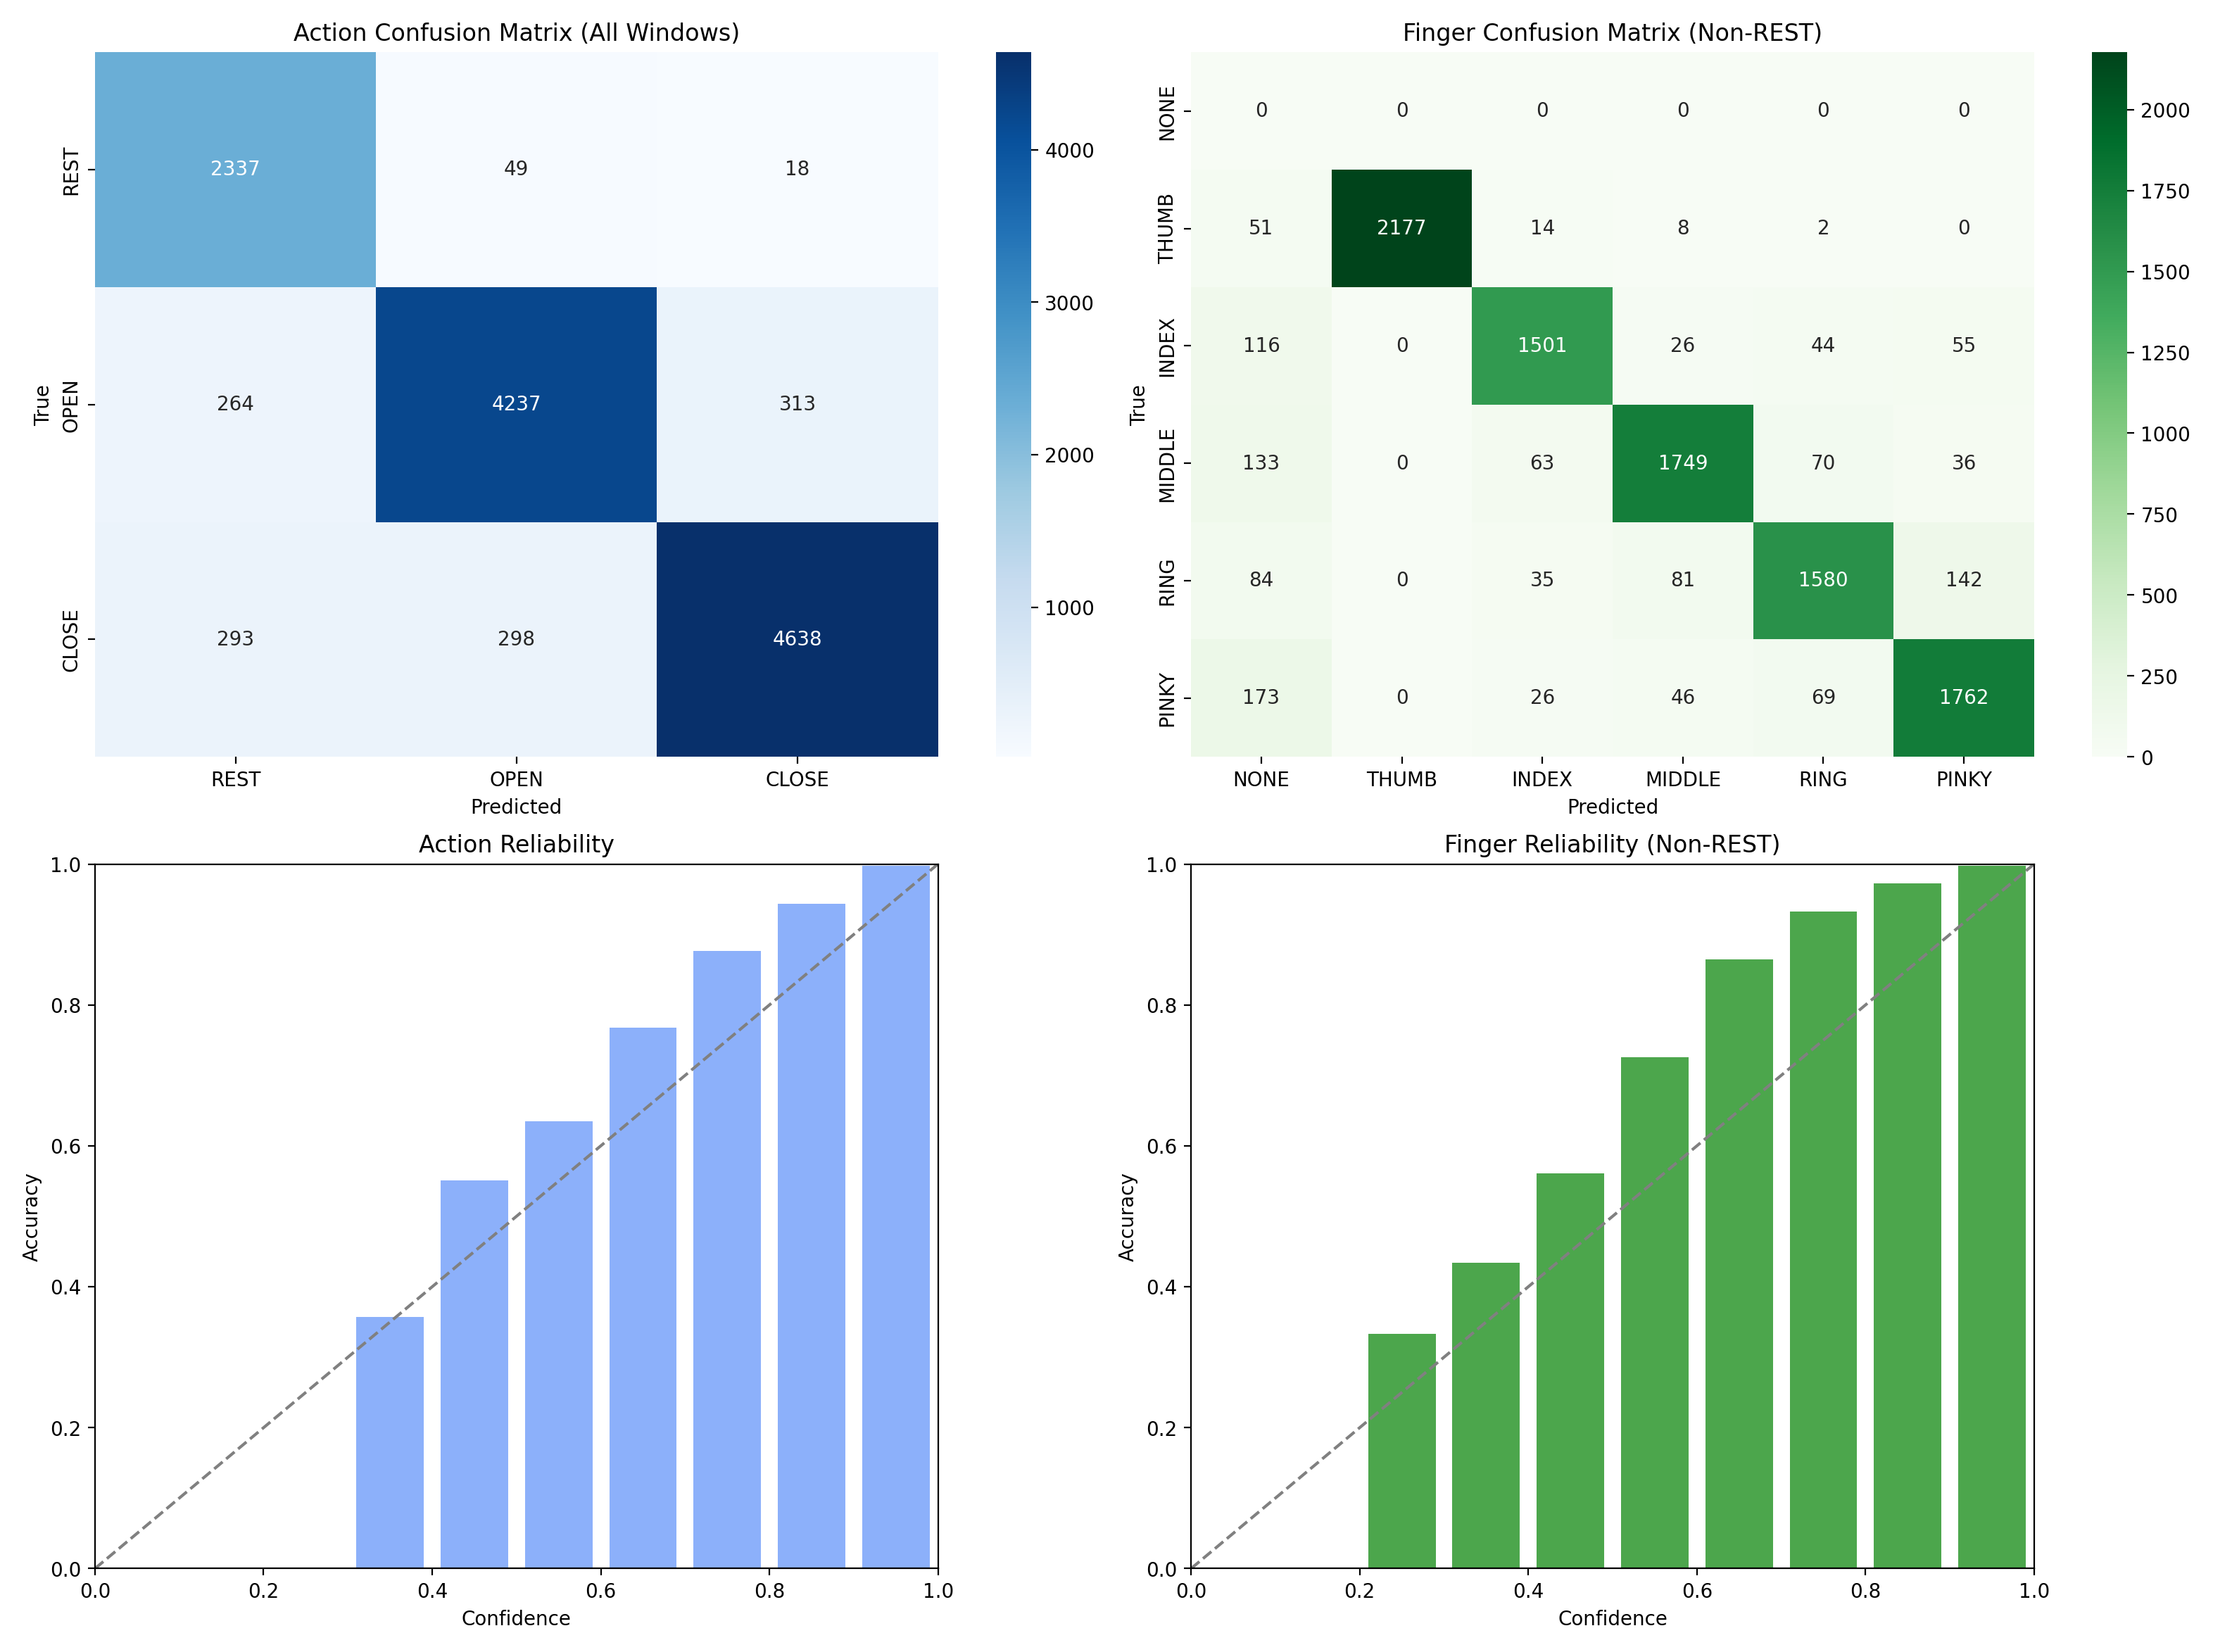
\includegraphics[width=\linewidth]{../paper_figures/2-M16_combined_20260319_081200_pruned_rest_events_0_1_2_20260319_075520__mc_eval.png}
\\\footnotesize (a) Step~3c reliability/calibration summary, including action and finger confusion matrices (2-M16).
\end{minipage}
\begin{minipage}[b]{0.49\linewidth}\centering
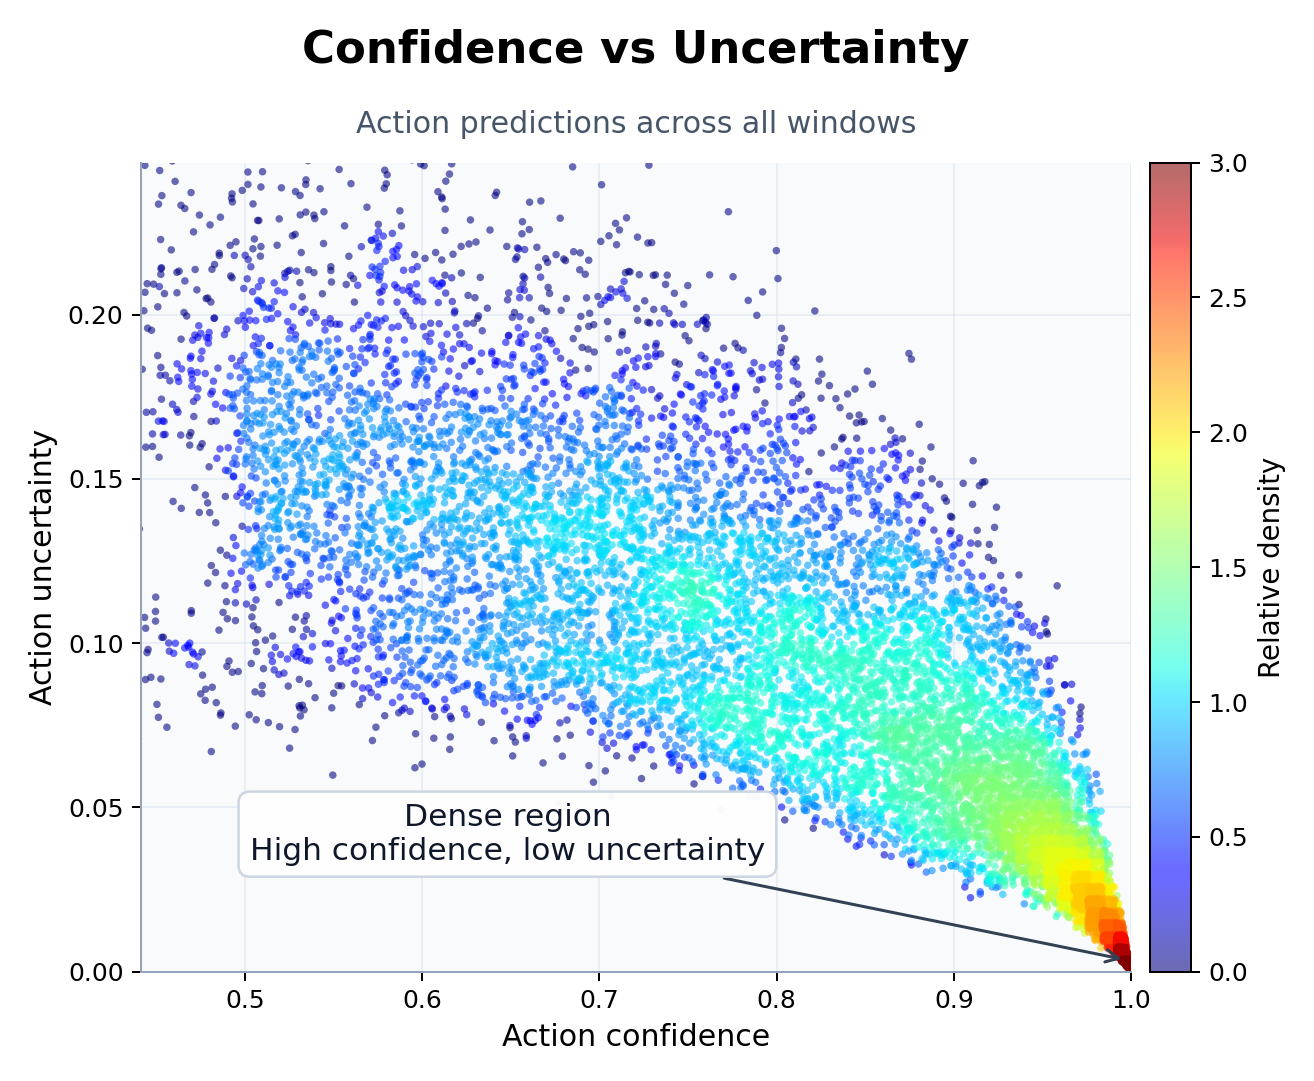
\includegraphics[width=\linewidth]{../paper_figures/2-M16_combined_20260319_081200_pruned_rest_events_0_1_2_20260319_075520__mc_scatter.png}
\\\footnotesize (b) Supporting MC-dropout confidence--uncertainty view (2-M16).
\end{minipage}
\caption{Representative Step~3c evaluation outputs for the featured 2-M16 run. The reliability/calibration panel includes action and finger confusion matrices, while the confidence--uncertainty panel summarizes MC-dropout behavior across windows.}
\label{fig:featured-evaluation}
\end{figure*}

\begin{figure}[t]
\centering
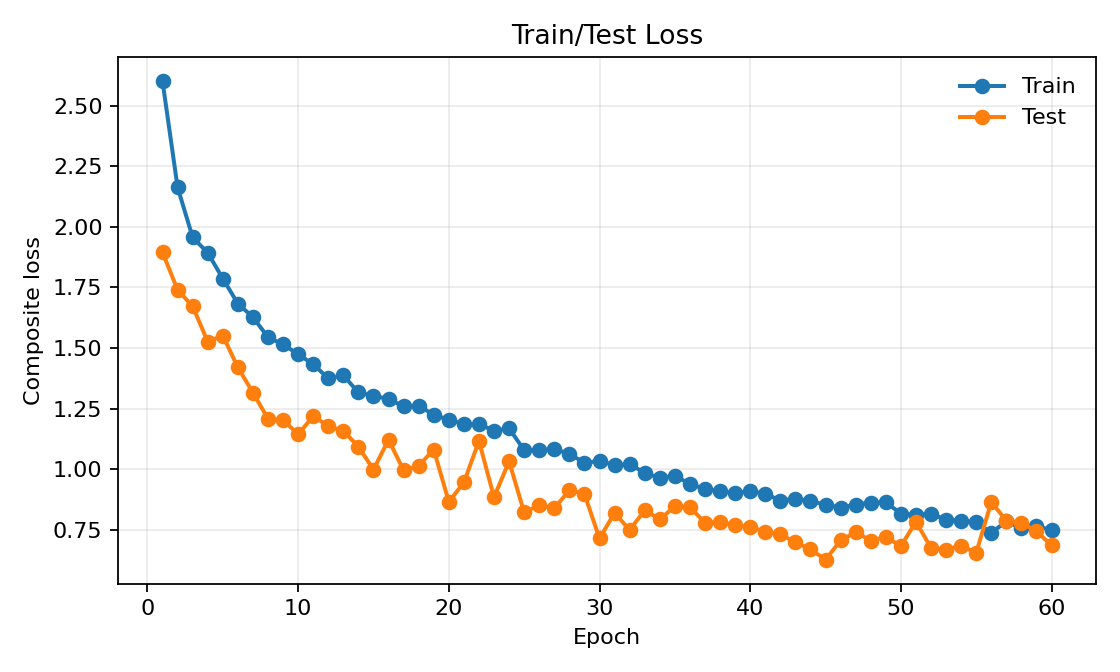
\includegraphics[width=\linewidth]{../paper_figures/2-M16_combined_20260319_081200_pruned_rest_events_0_1_2_20260319_075520__loss_curve.png}
\caption{Additional training-dynamics validation for the featured recipe: train/test composite loss by epoch (featured recipe rerun recorded history). The curve is generated only from recorded per-epoch history and is not reconstructed from final metrics.}
\label{fig:featured-loss-curve}
\end{figure}



\subsection{Per-Class Behavior}
Per-class test accuracies and counts are derived from the saved per-window prediction bundles and reported separately for action and finger labels in Tables~\ref{tab:perclass-action} and~\ref{tab:perclass-finger}. The aggregate results are not carried by one dominant class alone. THUMB is near ceiling at 99.57\%, INDEX remains strong at 94.50\%, and PINKY reaches 89.57\%, while MIDDLE and RING are lower at 79.01\% and 65.48\%, respectively. RING is the main outlier at 65.48\%, and its lower accuracy is discussed in Section~\ref{sec:discussion} as a likely consequence of finger-specific representational overlap, low-density channel placement, and subject-specific signal geometry. This asymmetry matters because a single average finger-accuracy value hides which degrees of freedom remain fragile.

\begin{table*}[t]
\centering
\caption{Per-class accuracies on the test split (computed from saved per-window predictions).}
\label{tab:perclass}
\begin{tabular}{lllrr}
\toprule
Task & Subject & Class & Count & Accuracy (\%) \\
\midrule
Action & 1-M16 500 & REST & 114 & 0.88 \\
Action & 1-M16 500 & OPEN & 1171 & 88.98 \\
Action & 1-M16 500 & CLOSE & 1363 & 73.81 \\
Finger (non-REST) & 1-M16 500 & THUMB & 651 & 95.39 \\
Finger (non-REST) & 1-M16 500 & INDEX & 551 & 85.12 \\
Finger (non-REST) & 1-M16 500 & MIDDLE & 526 & 91.83 \\
Finger (non-REST) & 1-M16 500 & RING & 460 & 70.87 \\
Finger (non-REST) & 1-M16 500 & PINKY & 346 & 82.95 \\
Action & 2-M16 & REST & 169 & 79.88 \\
Action & 2-M16 & OPEN & 789 & 90.87 \\
Action & 2-M16 & CLOSE & 1082 & 89.65 \\
Finger (non-REST) & 2-M16 & THUMB & 438 & 96.58 \\
Finger (non-REST) & 2-M16 & INDEX & 325 & 89.23 \\
Finger (non-REST) & 2-M16 & MIDDLE & 343 & 86.01 \\
Finger (non-REST) & 2-M16 & RING & 393 & 84.73 \\
Finger (non-REST) & 2-M16 & PINKY & 372 & 91.67 \\
\bottomrule
\end{tabular}
\end{table*}



Action-class behavior also deserves context. For 2-M16, REST accuracy is high (98.37\%) but is estimated from \FeaturedNRest{} REST test windows out of \FeaturedNTest{} total test windows, so the denominator remains modest relative to the non-REST split. Continuous windowing expands the number of REST windows, but the REST subset remains small relative to OPEN and CLOSE. This is why the pseudo-live false REST actuation rate is reported separately from REST test accuracy: it directly measures whether REST-labeled replay windows would have produced unsafe movement commands.

\subsection{Archive Scope}
The project archive contains an earlier single-session 1-M16 run, but this manuscript does not use it for quantitative comparison because its dataset construction and evidence chain are not matched to the featured 2-M16 bundle. A matched multi-subject analysis should wait until the archive contains prospectively paired dataset construction, filtering rules, and replay outputs across subjects.

\subsection{Statistical Interpretation}
We report 95\% confidence intervals (Wilson score) for action accuracy over $n_{test}$ windows and for finger accuracy over $n_{non\text{-}REST}$ windows in Table~\ref{tab:perf}. These intervals reflect finite test-set uncertainty under an i.i.d.\ window assumption; they do not account for temporal correlation induced by overlapping windows and event segments, which narrows the effective sample size. Percentile bootstrap intervals computed from the same saved correctness vectors closely tracked the Wilson intervals and did not change the interpretation, so the main paper reports a single interval family.

\section{Discussion}
\label{sec:discussion}
AlphaHand preserves finger-level decoding through actuation-grade command logic. Held-out classification alone can overstate practical utility, so the central result is not only that the featured run reaches high offline accuracy, but that it remains usable after deterministic decoding and pseudo-live safety gates. Here, the featured run preserves \FeaturedJointAcc\% deterministic joint action--finger accuracy, then keeps false REST actuation to \FeaturedFalseActuationRateRest\% under pseudo-live replay while hitting \FeaturedReplayEventHitRate\% of movement events. The deployment decoder therefore reduces throughput without eliminating the useful finger-level signal.

The replay operating point favors precision over throughput. This is appropriate for an early assistive-control prototype because false movement can be more disruptive than missed movement, but it also means the system is not yet optimized for user-perceived responsiveness. Precision is high (\FeaturedReplayPrecision\%), while window-level send recall is lower than held-out accuracy because the denominator counts overlapping windows, not intended movements. In practical terms, the current gate suppresses uncertain commands rather than risking frequent false movements; in the featured replay stream, only \FeaturedReplayFalseActuationCount{} actuation-sent windows occurred on \FeaturedReplayRestWindows{} true REST windows. For an early physical assistive device, this is the safer side of the precision--recall tradeoff.

The same operating point still limits usability. A low window-level send recall means many overlapping movement windows do not emit commands, but it should not be read as classifier accuracy. A better usability target is event-level hit rate with first-command latency: did each intended movement receive at least one correct command quickly enough to feel responsive? The current replay hit \FeaturedReplayEventHitRate\% of movement events with \FeaturedReplayLatencyMedianMs{} ms median and \FeaturedReplayLatencyPNinetyFiveMs{} ms p95 first-command latency. Threshold relaxation, shorter stability requirements, and cooldown tuning can increase throughput, but the expected cost is lower precision and more false or redundant actuation. Future deployment studies should identify the operating point that users find acceptable, rather than assuming the safest offline gate is clinically useful.

The per-finger asymmetry is equally important. THUMB, INDEX, and PINKY are strong in the featured run, while MIDDLE and RING remain less stable. RING is the clearest example of this fragility. Its lower accuracy may reflect overlap between middle/ring motor representations, mechanically coupled finger movement during data collection, or the absence of central motor-strip electrodes that would better separate neighboring digits. With only TP9, AF7, AF8, and TP10, none of the recording sites lies over the central hand area typically sampled by C3/C4/Cz-style motor electrodes. The model is therefore decoding finger intent from a lateral frontal/temporal view of the sensorimotor system rather than direct coverage of the central strip. The observed asymmetry is plausibly driven by cortical representational overlap, limited channel coverage, and lower signal-to-noise ratio for some fingers, not just by classifier capacity.

The difference from Xiao and Ding's 39.7\% five-finger result should not be read as four dry electrodes outperforming 128-channel EEG. Their high-density study used a different task, feature family, and validation setting, while AlphaHand reports subject-specific, action-conditioned active-finger accuracy and then imposes REST/NONE command logic. The action/finger factorization, REST definition, and conservative actuation gates change both the numerator and denominator. The useful comparison is therefore mechanistic rather than competitive: Xiao and Ding show that EEG can carry finger-specific spectral structure under rich sensing, while AlphaHand asks whether enough subject-specific structure remains in a sparse consumer montage to drive a conservative command path. The present results suggest that the answer can be yes for a trained subject and a tightly bounded deployment setting.

Future validation should lock the preprocessing, pruning, model-selection, calibration, and replay policies before data collection, then test whether command-path precision and event-level responsiveness persist across unfamiliar users and repeated sessions.

\subsection{Limitations}
\label{sec:limitations}
Several limitations bound the current evidence.

\textit{Statistical limitations.} Overlapping windows create temporal dependence, so Wilson intervals assume independent windows that the extraction procedure does not fully provide. Informative trial IDs are unavailable in the saved bundles, preventing trial-level aggregation and cleaner effective-sample-size estimates. The effective sample size is therefore likely smaller than the raw window count.

\textit{Dataset limitations.} Only one complete deployment evidence chain is reported quantitatively; the broader consented archive is more diverse, but those recordings do not yet provide matched datasets with trained checkpoints, calibration outputs, and replay outputs. The featured 2-M16 participant was a study-team self-subject, so familiarity with the task and recording protocol may inflate performance relative to users unfamiliar with the protocol. The featured dataset also uses targeted REST pruning, and the representative checkpoint was selected retrospectively from an archive using evidence-chain completeness and deployment safety. Prospective locked-protocol evaluation is needed before treating these numbers as unbiased performance estimates.

\textit{Physiological and EEG artifact limitations.} Muse 2 lacks dedicated EMG/EOG channels, and no post-hoc ICA-based artifact rejection was available, so protocol-level artifact reduction and stream-health monitoring cannot fully rule out non-cortical artifacts such as movement, muscle, gaze, or connectivity artifacts. The low-density electrode placement also does not directly cover C3/C4/Cz motor areas, limiting anatomical specificity for neighboring fingers.

\textit{Deployment limitations.} Pseudo-live replay is not a full live-loop validation. Dedicated live-loop latency logs are \NotAvailable{}, so replay-time summaries cannot substitute for a full end-to-end timing audit. User-level command utility has not yet been tested prospectively.

\section{Conclusion}

AlphaHand demonstrates that consumer EEG can support more than coarse grasp detection in a subject-specific setting. The strongest run reaches \FeaturedActionAcc\% held-out action accuracy and \FeaturedFingerAcc\% deployment-consistent finger accuracy, and the same bundle remains credible under deterministic evaluation and pseudo-live replay. The present contribution is an auditable end-to-end demonstration of finger-level control from a four-channel headset, with scope and limitations explicitly documented. Achieving broader clinical relevance will require prospective multi-session cohorts, explicit artifact-rejection logging, and live-loop validation that jointly reports accuracy, latency, false actuation, and user-level command utility.

\section*{Data and Code Availability}

Code, trained outputs, and derived datasets will be made available where consent and privacy constraints permit. Raw recordings containing participant EEG are governed by the study consent protocol and are not released without appropriate safeguards.

\section*{Author Contributions and Funding}

Jonathan Davanzo served as first author and lead researcher for AlphaHand. He personally funded the project and led the project conception, software implementation, system construction, experimental pipeline, model training and evaluation workflow, and manuscript preparation.

\bibliographystyle{IEEEtran}
\bibliography{references}

\end{document}
